\chapter{Preliminares}


% https://it.wikipedia.org/wiki/Isosuperficie#cite_note-:2-3
\section{Funciones de distancia con signo\label{sec:fds}}

Una función de distancia con signo (\textit{FDS}) se trata de una aplicación \(f: \mathbb{R}^n\longrightarrow \mathbb{R}\). Esta aplicación transforma un punto \(\Vec{p}\) de un espacio multidimensional en un valor. En particular, trabajaremos con espacios bidimensionales y tridimensionales, donde el valor devuelto es la distancia mínima con signo hasta un punto \(\Vec{q}\) de un perímetro o una superficie \(S\). 
\[f(\Vec{p})=\pm min_{\Vec{q}\in S}\vert\vert \Vec{p}-\Vec{q} \vert\vert , \Vec{p} \in \mathbb{R}^n, n\in \{2,3\}\]
El signo de esta distancia contiene información sobre la escena: con una distancia positiva, nos encontramos en el exterior de una figura, en caso de ser cero, nos encontraremos en la superficie (corteza) \(S\), por último, con una distancia negativa, estaremos dentro del volúmen de la figura, que en positivo representa la profundidad del punto respecto de la corteza. 

\begin{definition}
	Sea \(f:\mathbb{R}^2\longrightarrow\mathbb{R}\), una función de distancia con signo, definimos como \textit{isoperímetro}, \(L=\{\Vec{p} \vert f(\Vec{p})=0\}\).
\end{definition}

\begin{definition}
	Sea \(f:\mathbb{R}^3\longrightarrow\mathbb{R}\), una función de distancia con signo, definimos como \textit{isosuperficie}, \(S=\{\Vec{p} \vert f(\Vec{p})=0\}\).
\end{definition}

Para esta última definición, presentaremos un algoritmo de trazado de escena denominado \textit{Spheremarcher}\ref{sec:spheremarching}.
\newpage
\section{La normal de una isosuperficie \label{sec:normal}}

Vamos a presentar un teorema esencial para el cálculo de la normal de una superficie, cuya demostración propuesta por  \cite{goldman2005curvature} (p. 641-642). Esta es fundamental para la confección de una escena, especialmente en un modelo de iluminación\ref{ch:iluminacion}.

\begin{theorem}
	El vector gradiente \(\nabla f(x_0, y_0, z_0)\)  es perpendicular a la curva de la tangente de una \textit{isosuperficie} en el punto \(\Vec{p}=(x_0, y_0, z_0)\).
\end{theorem}

En realidad, nos quiere decir que la normal de una \textit{isosuperficie} es proporcional a su gradiente o exacta en caso de su posterior normalización\footnote{Decimos que un vector está normalizado cuando su módulo es exactamente \(1\) .}, que denotaremos:
\[norm:\mathbb{R}^n\longrightarrow\mathbb{R}^n, norm(\Vec{v})=\dfrac{\Vec{v}}{\vert\vert v \vert\vert}\]
%Su demostración está basada en el concepto del plano tangente.\\\\
% https://tutorial.math.lamar.edu/classes/calciii/gradientvectortangentplane.aspx
Se define formalmente el gradiente de una función tridimensional, como:
\[ \nabla f(x, y, z)= < \partial_x f, \partial_y f, \partial_z f, > \]
donde \enquote{\(\partial_{x_i}\)} es la derivada parcial de una función respecto de la variable \(x_i\). Definida por: 
\[ \partial_{x_i}f=\lim_{\epsilon\longrightarrow 0}\dfrac{f(x_0,\cdots,x_i+\epsilon,\cdots,x_n)-f(x_0, \cdots, x_n)}{\epsilon} \]
Se puede aproximar computacionalmente, tomando \(\epsilon\) próximo a \(0\), por ejemplo, \(\epsilon = 0.001\).
Finalmente, definimos el gradiente computado como:
\[
\Vec{n}=norm(\nabla f(x, y, z))\approx norm\left(
\stretchleftright[1000]{\langle}
{\begin{array}{c}
\dfrac{f(x+0.001,y,z)-f(x,y,z)}{0.001}\\
\dfrac{f(x,y+0.001,z)-f(x,y,z)}{0.001}\\
\dfrac{f(x,y,z+0.001)-f(x,y,z)}{0.001} \end{array}}
{\rangle}\right)
\]

\section{Homeomorfismos sobre [0, 1]}

Vamos a definir una aplicación que nos ayudará a deformar funciones de manera continua. Esta aplicación nos será muy útil para manipular las propiedades de la escena, por ejemplo, la intensidad lumínica en nuestro modelo de iluminación, transformación de color, velocidad de un objeto de un punto a otro, etc.

\begin{definition}
    Sea una función \(f:X\longrightarrow Y\), diremos que esta es homeomórfica, si y solo si:
    \begin{enumerate}
        \item \(f\) es continua.
        \item \(f\) es biyectiva.
        \item \(f^{-1}\) es continua.
    \end{enumerate}
\end{definition}
Restringimos los homeomorfismos a \(X=Y=[0,1]\) con \(f(0)=0\) y \(f(1)=1\). Esta restricción es importante para valores normalizados, ya que aseguramos que sus extremos quedan invariantes.\\\\
Supongamos una imagen en escala de grises con un único canal. El canal acepta un intervalo real \([0, 1]\), donde el color negro es el \(0\) y el blanco, el \(1\). Por ejemplo, definimos nuestro \textit{homeomorfismo}:
\[f(x)=x^8, x \in [0, 1]\]
Así, podemos comprobar que esta función cumple con las propiedades descritas anteriormente. En la siguiente representación podemos distinguir una serie de exponentes desde 1 hasta 11, en \textcolor{blue}{azul} nuestra función \(f\).
\begin{figure}[H]
    \centering
    \captionsetup{justification=centering}%,margin=2cm
    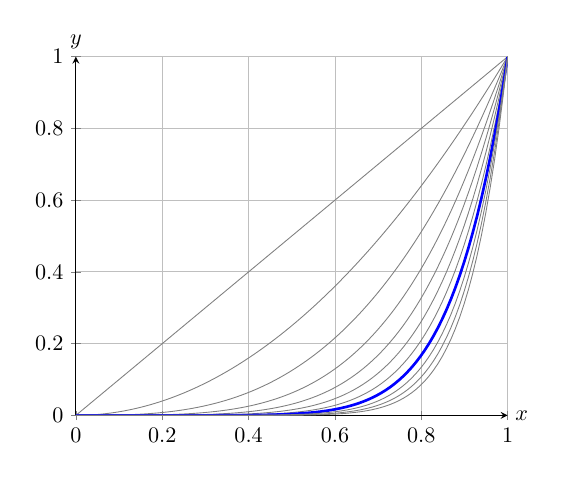
\begin{tikzpicture}[scale=0.8]
        \begin{axis}[
            % Function Properties
            domain=0:1,
            samples=100,
            % Grid Properties
            grid=both,
            % X, Y Coordinates
            axis lines=left,
            compat=newest,
            xlabel=$x$, xlabel style={at={(1,0)}, anchor=west},
            ylabel=$y$, ylabel style={rotate=-90,at={(0,1)}, anchor=south}
        ]
            \addplot[gray] (x,x);
            \addplot[gray] (x,x^2);
            \addplot[gray] (x,x^3);
            \addplot[gray] (x,x^4);
            \addplot[gray] (x,x^5);
            \addplot[gray] (x,x^6);
            \addplot[gray] (x,x^7);
            \addplot[blue, very thick] (x,x^8);
            \addplot[gray] (x,x^9);
            \addplot[gray] (x,x^10);
            \addplot[gray] (x,x^11);
        \end{axis}
    \end{tikzpicture}
    \caption{Gráfica de los distintos \(f_n(x)=x^n, n\in\{1,\cdots,11\}\subset \mathbb{N}\) } \label{fig:M1}
\end{figure}
Los valores inferiores a \(0.6\) se transforman a valores próximos a \(0.0\), oscureciendo los tonos grises, manteniendo los colores claros.
\begin{figure}[H]
  \centering
  \captionsetup{justification=centering}%,margin=2cm
  \subfloat[Imagen original]{\includegraphics[width=0.45\textwidth]{secciones/imagenes/preliminars/pol8-img-left.png}}
  \hfill
  \subfloat[\(f(x)=x^8\) sobre la imagen original]{\includegraphics[width=0.45\textwidth]{secciones/imagenes/preliminars/pol8-img-right.png}}
  \caption{A la izquierda una imagen con un canal \([0,1]\). A la derecha, la misma imagen, pero aplicado el \textit{homeomorfismo} \(f\).}
  \label{fig:homeomorphism}
\end{figure}
En código: \url{https://www.shadertoy.com/view/wljfR1}

\section{Homotopías}
% Nota pie
En esta última sección, vamos a ver una aplicación matemática que es utilizada para animación y texturización. Vamos a centrarnos en el intervalo \([0, 1]\), aunque podemos trabajar sobre cualquier intervalo, antes deberemos normalizar y  finalmente, reescalar.

\begin{definition}
    Dadas dos aplicaciones \(f, g:X\longrightarrow Y\), continuas, decimos que son homotópicas. Si existe una aplicación \(H\), también continua, tal que:
    \[ H:X\times[0,1]\longrightarrow Y \]
    \[ H(x, 0)=f(x) \]
    \[ H(x, 1)=g(x) \]
\end{definition}
% nota pie
\begin{definition}
    Claramente \(H\) es una homotopía, llamaremos función de mezcla lineal\label{def:mix}\footnote{Se utiliza este concepto en la documentación oficial, sección \enquote{8.3 Common Functions}} a la homotopía:
    \[H(x, t)=(1-t)\cdot f(x) + t\cdot g(x)\]
\end{definition}

Como podemos observar,  la última definición es una homotopía, ya que, la suma de dos funciones continiuas es siempre continua y los extremos resultan \(f(x)\) y \(g(x)\), respectivamente.\\\\
Como \(t\in[0,1]\), podemos aplicar un \textit{homeomorfismo} \(p(t)\) y tener así, una versión más general.
    \[H(x, t')=H(x, p(t))=(1-p(t))\cdot f(x) + p(t)\cdot g(x)\]
Veamos un ejemplo, supongamos que \(f(x)\) y \(g(x)\) son los colores de una imagen 3-canal y como \(t\), una tercera imagen con un canal \([0,1]\), que actuará como máscara.
\begin{figure}[H]
  \centering
  \captionsetup{justification=centering}%,margin=2cm
  \subfloat[Imagen \(f(x)\)]{\includegraphics[width=0.30\textwidth]{secciones/imagenes/preliminars/texture-wall.png}}
  \hfill
  \subfloat[Imagen \(g(x)\)]{\includegraphics[width=0.30\textwidth]{secciones/imagenes/preliminars/texture-galaxy.png}}
  \hfill
  \subfloat[Máscara \(t\)]{\includegraphics[width=0.30\textwidth]{secciones/imagenes/preliminars/mask.png}}
  \caption{Imagen \(f(x)\), Imagen \(g(x)\) y Máscara \(t\)}
  \label{fig:textures}
\end{figure}
Los resultados obtenidos con diferentes homomorfismos.
\begin{figure}[H]
  \centering
  \captionsetup{justification=centering}%,margin=2cm
  \subfloat[Mezcla con el homeomorfismo \(p(t)=t\)]{\includegraphics[width=0.45\textwidth]{secciones/imagenes/preliminars/masking-result-1.png}}
  \hfill
  \subfloat[Mezcla con el homeomorfismo \(p(t)=t^4\)]{\includegraphics[width=0.45\textwidth]{secciones/imagenes/preliminars/masking-result-2.png}}
  \caption{Mezcla con distintos homomorfismos.}
  \label{fig:homotopies}
\end{figure}

Un ejemplo práctico: \url{https://www.shadertoy.com/view/wt2fR1}